%!TEX root=report.tex

\subsection{OLS AR(1)}
The difference between standard OLS and the proposed model for OLS with autocorrelated residuals was examined for a multitude of different locations on the globe.
Now, since the AR part of the model requires equidistant time series a linear interpolation was used to fill in the many gaps that existed in the data. 
Sadly, however, even when using interpolated time series there seemed to be very little difference between the two models. This was a bit surprising since the $\rho$ estimate almost always was close to $0.9$ and in some cases even higher. 

Since the difference between models were negligible, we find that it suffices to show the results for just one such location (in this case (lon,lat)$=(24,134)$).
Firstly a visual representation of the differences:

\begin{figure}[H]
\centering
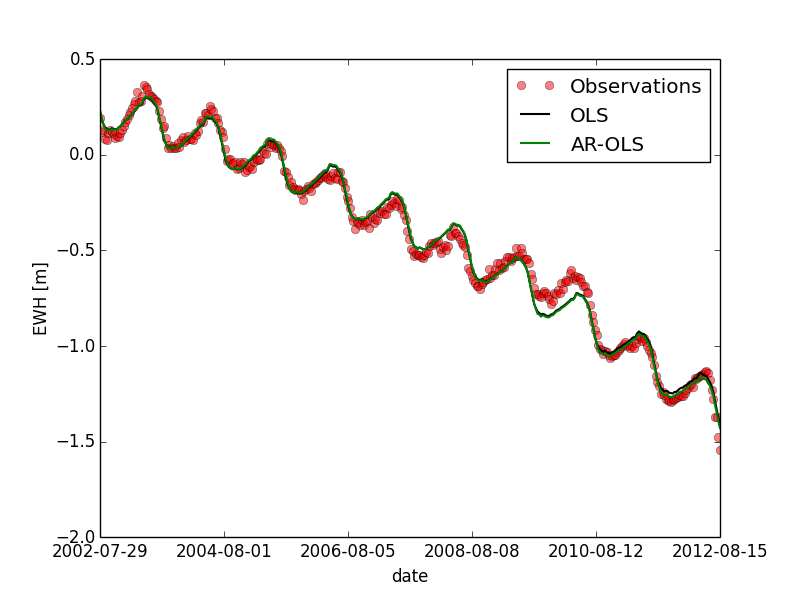
\includegraphics[width=1.0\linewidth]{figures/ols-AR(1)-24-134}
\caption{OLS. vs OLS with autocorrrelated residuals - comparison made for the west coast of Greenland. Here $\hat{\rho}\approx0.894$.}
\end{figure}

Secondly, follows an overview of the models:
\begin{tabular}{l || c |  r}[H]
 & OLS & OLS-AR(1) \\ \hline
$R^2$ & 0.990 &0.875 \\
AIC & -1149 &-1742 \\
Durbin-Watson & 0.208 & 2.354
\end{tabular}\\\\
On the positive side the Durbin-Watson test suggest that the model improved  ($0\ge D\ge 4$. $D<<2$ implies positive autocorrelation between the residuals while $D>>2$ implies negative autocorrelation). 
As discussed in the theory section, when $D<<2$ model estimates tend to be too optimistic.
 This is seen in the table above as well as in the estimated t-scores (not shown here). 
\\
Seeing as the OLS overestimates its performance and the model predictions look visually similar(this is due to the fact that the biggest absolute difference in $\beta$ coefficients is $10^-3$) it is hard to objectively identify the best model.
 However, if one were pressed to conclude something it might be that the OLS-AR(1) model most likely provides a more realistic estimate of the model performance than pure OLS. 
So to recap, the $\beta$-vector estimates were found to be almost identical and the only improvement offered by OLS-AR(1) is given by more precise p-values.
